% \documentclass[11pt]{article}

% \parskip 6pt % 1pt = 0.351 mm
% \parindent 0pt

% \usepackage{graphicx}				% Use pdf, png, jpg, or eps§ with pdflatex; use eps in DVI mode
% \usepackage[draft]{fixme}

% \newcommand{\comp}[1]{\emph{#1}}

% \begin{document}


% 1. Describe general SW-learning architecture

% 2. Link it to the design of the "core components"

% 3. Link the different components to the tasks in the WP

% 4. Link to class diagrams in the appendix
 
% 5. Summary of the parts of the design that has been implemented



\subsection{The learning module}

The core components of the modeling framework has been designed and implemented to facilitate an easy
integration with the inference and learning modules developed as part of Work packages 3 and 4. Figure~\ref{fig:design-learning} 
shows a high-level overview of the key components of the AMIDST software tool that is directly
related to learning; these learning-related components are connected to the framework core (see Section~\ref{sec:core-module}) through the \comp{Inference}
component and the \comp{PGM} component (shown using boxes with sharp corners).   

  \begin{figure}[htbp]
    \centering
    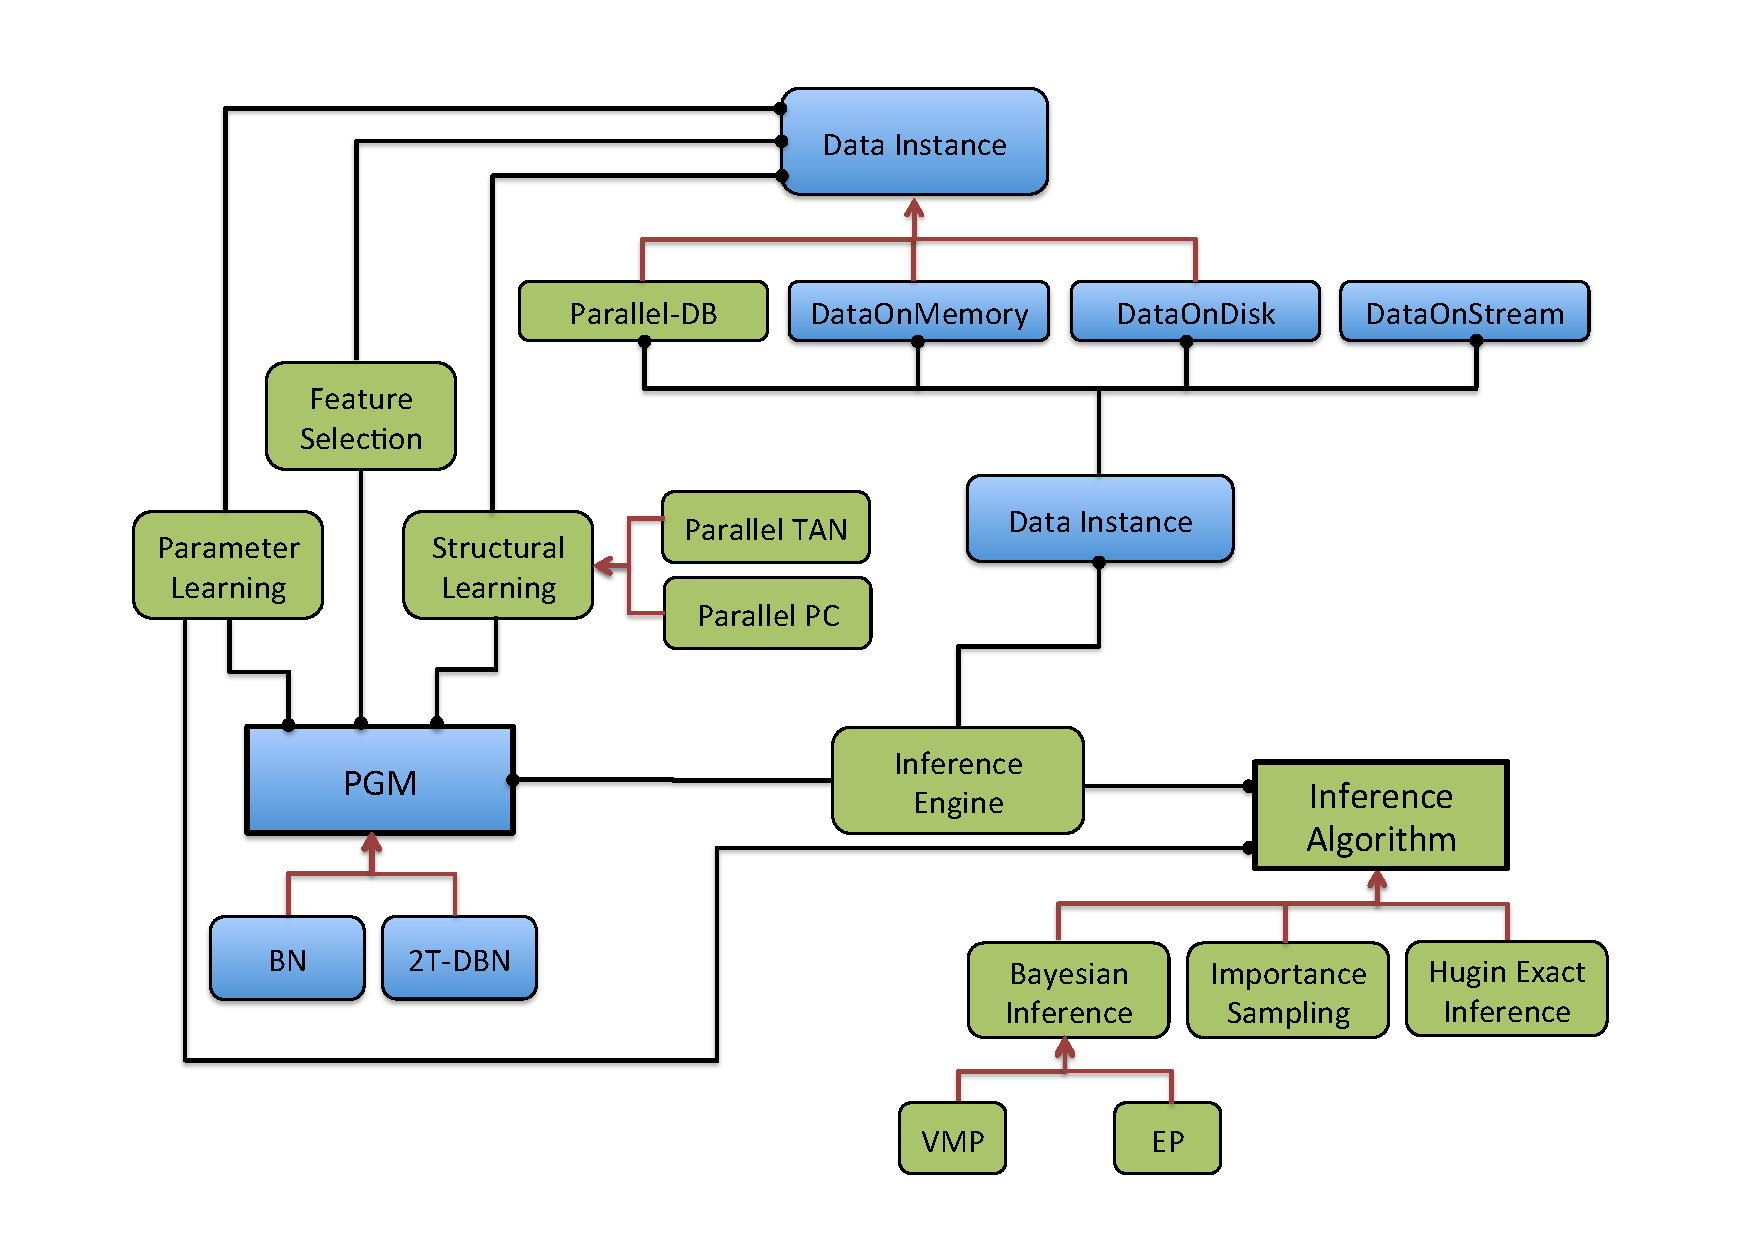
\includegraphics[width=1.05\linewidth]{design-learning2}
    \caption{Illustration of the design of the software components related to model learning. }
    \label{fig:design-learning}
  \end{figure}

In the AMIDST framework we consider two types of data sources for learning: i) Streaming data, where data arrives at high
frequency with no storage of historical data (except for data in the most recent past, which is stored in a
buffer), and 2) static databases that simply correspond to traditional databases. The database support is
realized by a general database component (\comp{Database}) that defines the database interface from which more
specialized databases (\comp{DataOnMemory}, \comp{DataOnDisk}, and \comp{ParallelDatabase}) can be derived:
\begin{itemize}
\item \comp{DataOnMemory} implements database functionality for data sets that can be loaded into main memory.
\item \comp{DataOnDisk} provides functionality for handling datasets too large to be loaded in main memory.
\item \comp{Parallel-DB} implements a distributed database.
\end{itemize}
The employed design is intended to support future users and developers of the AMIDST toolbox in the
potential design
and implementation of other
database specifications; the only restriction being that new database components should implement the interface defined by the
\comp{Database} component. 

Functionality for handling data streams is implemented by the \comp{DataOnStream} component that allows data
to be \emph{pushed} to the AMIDST system (in contrast to a pull-approach that is standard when dealing with static
database). To allow for variation in the run-time performance of the system a buffer component
(\comp{Buffer}) is needed for storing the most recent unprocessed cases. Each of the data sources are
furthermore connected to the \comp{Data Instance} component. This component consists of a single class
that can represent a particular evidence configuration, such as the observed values of a collection of variables at
time $t$ or a particular row in a database. 

Implementations of structural learning algorithms will be realized through the \comp{Structural learning}
component and its specialized sub-classes. The design includes components for supporting PC and TAN
learning in a parallel setting (cf.\ Task 4.1). Currently, the corresponding implementation supports standard PC
learning and parallel TAN learning by interfacing to the Hugin API. 

As described in Section~\ref{sec:learningAsInference} we pursue a fully Bayesian approach for doing parameter learning in the AMIDST
framework (cf.\ the activities in Task 4.2 and Task 4.4). This, in turn, means that parameter learning reduces
to the task of inference for which  we
plan to consider two approaches: variational message passing (positioned in a variational Bayes framework and implemented in the \comp{VMP} component) and
expectation propagation (implemented in the \comp{EP} component); both components are derived from the more
general \comp{Inference} component. Particular efficient
implementations of both variational inference and expectation propagation can be realized when the distribution families of the models are
conjugate-exponential. In this case the inference operations can be further supported by specifying the
exponential distributions using their natural parameters, see Section~\ref{sec:learningAsInference}. These improvement are realized
through tailored exponential family implementations of the standard distributions that are part of the AMIDST framework
(such as the conditional linear Gaussian distribution). Note that the design of this parameter learning part of
the overall AMIDST framework is flexible in the sense that it easily accommodates potential future learning-based extensions of
the framework, e.g., Bayesian learning based on importance sampling or maximum likelihood learning using the
expectation maximization algorithm (see also
Section~\ref{sec:learningAsInference}).   

Variable selection is handled in the corresponding component in Figure~\ref{fig:design-learning}, which is
connected to both the model component (\comp{PGM}) and the \comp{Database} component. 

The high-level design description above provides an overview of the current design of the AMIDST software
framework with particular focus on the components that are directly related to model learning. The current
status of the software implementation in relation to this design is as follows:
\begin{itemize}
\item The core components (marked as blue in Figure~\ref{Figure:ToolboxBasicStructure}) has been implemented. This includes data structures
  for variables, graphs, Bayesian networks, dynamic Bayesian networks, key distributions such as multinomial
  and conditional linear Gaussian distributions represented in both standard form and as exponential families.
\item Components defining data source management functionalities have been implemented, which includes support
  for handling static database (on disk and in memory) as well as streaming data.   
\item Methods for transforming AMIDST models to and from Hugin has been implemented based on the Hugin API.  
\end{itemize}
Please see the appendix for the class diagrams for the implemented components.



\emph{Remark: The implementation is still ongoing and will continue so until the deliverable is
  submitted. Thus I expect that we will be able to expand the above list a bit. In particular, I know that
  there is currently work going on to provide parallel TAN learning in the AMIDST toolbox by calling the Hugin
  API. This would also be demonstrated at the review meeting.}  















%\end{document}

%%% Local Variables: 
%%% mode: latex
%%% TeX-master: "D41-report"
%%% End: 
